\documentclass{article}
\usepackage{graphicx}
\usepackage{tikz}
\usetikzlibrary{circuits.logic.US}

\title{Boolean Algebra and Logic Circuits: \\
       Exploring the Connection and Design Principles for Digital Logic Gates}
\author{Badger Code}
\date{\today}

\begin{document}
\maketitle

\section{Introduction}
Boolean algebra serves as the foundation of digital logic design, enabling the construction of complex circuits and systems from simple logic gates. This paper explores the connection between Boolean algebra and logic circuits, focusing on design principles for digital logic gates. We will delve into the fundamental concepts of Boolean algebra, discuss how logic gates implement Boolean functions, and present visual representations of logic gates.

\section{Boolean Algebra Basics}
Boolean algebra deals with binary variables and logic operations. The variables take on the values of 0 and 1, representing false and true, respectively. The three fundamental operations in Boolean algebra are \textit{AND}, \textit{OR}, and \textit{NOT}.

\subsection{Boolean Operators}
\begin{itemize}
    \item \textbf{AND:} Denoted by $\cdot$ or $\land$, the \textit{AND} operation returns 1 only if both inputs are 1; otherwise, it returns 0.
    \item \textbf{OR:} Denoted by $+$ or $\lor$, the \textit{OR} operation returns 1 if at least one input is 1; otherwise, it returns 0.
    \item \textbf{NOT:} Denoted by $'$ or $\lnot$, the \textit{NOT} operation negates the input. It returns 1 if the input is 0 and vice versa.
\end{itemize}

\section{Logic Gates and Boolean Functions}
Logic gates are physical implementations of Boolean functions, where inputs and outputs take binary values (0 or 1). Common logic gates include \textit{AND}, \textit{OR}, \textit{NOT}, \textit{NAND}, \textit{NOR}, and \textit{XOR} gates.

\subsection{AND Gate}
The \textit{AND} gate implements the \textit{AND} operation in Boolean algebra. Its output is 1 only when both inputs are 1.

\begin{center}
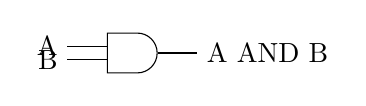
\begin{tikzpicture}
    \draw (0,0) node[and gate US, draw, logic gate inputs=nn] (AND) {};
    \draw (AND.input 1) -- ++(-0.5,0) node[left] {A};
    \draw (AND.input 2) -- ++(-0.5,0) node[left] {B};
    \draw (AND.output) -- ++(0.5,0) node[right] {A AND B};
\end{tikzpicture}
\end{center}

The output of the \textit{AND} gate is given by $A \cdot B$.

\subsection{OR Gate}
The \textit{OR} gate implements the \textit{OR} operation in Boolean algebra. Its output is 1 if at least one input is 1.

\begin{center}
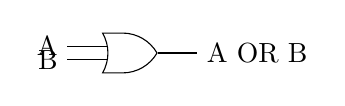
\begin{tikzpicture}
    \draw (0,0) node[or gate US, draw, logic gate inputs=nn] (OR) {};
    \draw (OR.input 1) -- ++(-0.5,0) node[left] {A};
    \draw (OR.input 2) -- ++(-0.5,0) node[left] {B};
    \draw (OR.output) -- ++(0.5,0) node[right] {A OR B};
\end{tikzpicture}
\end{center}

The output of the \textit{OR} gate is given by $A + B$.

\subsection{NOT Gate}
The \textit{NOT} gate implements the \textit{NOT} operation in Boolean algebra. It negates the input value.

\begin{center}
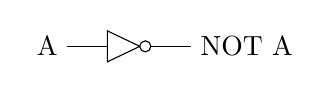
\begin{tikzpicture}
    \draw (0,0) node[not gate US, draw, logic gate inputs=n] (NOT) {};
    \draw (NOT.input) -- ++(-0.5,0) node[left] {A};
    \draw (NOT.output) -- ++(0.5,0) node[right] {NOT A};
\end{tikzpicture}
\end{center}

The output of the \textit{NOT} gate is given by $\overline{A}$ or $A'$.

\subsection{NAND Gate}
The \textit{NAND} gate is a combination of the \textit{AND} gate and the \textit{NOT} gate. Its output is the negation of the \textit{AND} operation.

\begin{center}
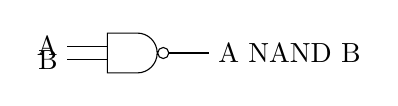
\begin{tikzpicture}
    \draw (0,0) node[nand gate US, draw, logic gate inputs=nn] (NAND) {};
    \draw (NAND.input 1) -- ++(-0.5,0) node[left] {A};
    \draw (NAND.input 2) -- ++(-0.5,0) node[left] {B};
    \draw (NAND.output) -- ++(0.5,0) node[right] {A NAND B};
\end{tikzpicture}
\end{center}

The output of the \textit{NAND} gate is given by $\overline{A \cdot B}$ or $(A \cdot B)'$.

\subsection{NOR Gate}
The \textit{NOR} gate is a combination of the \textit{OR} gate and the \textit{NOT} gate. Its output is the negation of the \textit{OR} operation.

\begin{center}
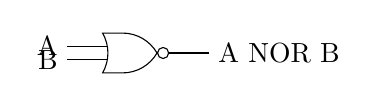
\begin{tikzpicture}
    \draw (0,0) node[nor gate US, draw, logic gate inputs=nn] (NOR) {};
    \draw (NOR.input 1) -- ++(-0.5,0) node[left] {A};
    \draw (NOR.input 2) -- ++(-0.5,0) node[left] {B};
    \draw (NOR.output) -- ++(0.5,0) node[right] {A NOR B};
\end{tikzpicture}
\end{center}

The output of the \textit{NOR} gate is given by $\overline{A + B}$ or $(A + B)'$.

\subsection{XOR Gate}
The \textit{XOR} gate, or exclusive OR gate, outputs 1 when the inputs are different and 0 when the inputs are the same.

\begin{center}
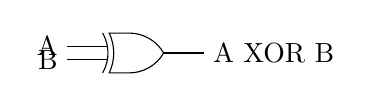
\begin{tikzpicture}
    \draw (0,0) node[xor gate US, draw, logic gate inputs=nn] (XOR) {};
    \draw (XOR.input 1) -- ++(-0.5,0) node[left] {A};
    \draw (XOR.input 2) -- ++(-0.5,0) node[left] {B};
    \draw (XOR.output) -- ++(0.5,0) node[right] {A XOR B};
\end{tikzpicture}
\end{center}

The output of the \textit{XOR} gate is given by $A \oplus B$.

\section{Design Principles for Digital Logic Gates}
The design of digital logic gates involves constructing circuits to implement Boolean functions efficiently and correctly.

\subsection{Gates Cascading}
Multiple logic gates can be cascaded together to build complex circuits. The output of one gate can serve as the input to another gate, enabling the implementation of more intricate Boolean functions.

\subsection{Boolean Algebra Simplification}
Boolean algebra can be used to simplify complex expressions, reducing the number of gates required in the circuit. Techniques like Boolean algebra laws, Karnaugh maps, and Quine-McCluskey method aid in simplifying Boolean expressions.

\section{Conclusion}
Boolean algebra and logic circuits are closely connected, enabling the design and implementation of complex digital systems. Logic gates serve as the building blocks of digital circuits, implementing Boolean functions and enabling the manipulation of binary data. Understanding the principles of Boolean algebra and logic gates is crucial for digital logic design and plays a central role in various electronic applications, including processors, memory units, and communication systems.

\end{document}